\section{Estudio de la situaci\'on actual}
\label{sec:estado-actual}

\subsection{Precursores: juegos de tablero.}

Los juegos de estrategia por turnos han estado presentes en la civilizaci\'on desde hace m\'as de 4000 a\~nos. Probablemente los m\'as representativos sean, precisamente, los m\'as antiguos: el tradicional Go chino, que ya se practicaba 2000 a\~nos antes del nacimiento de Cristo, o el ajedrez. Ambos fueron considerados durante siglos mucho m\'as que simples entretenimientos y en la antigua civilizaci\'on china la maestr\'{\i}a en el Go supon\'{\i}a la mejor muestra de erudici\'on de un hombre culto.\\

\begin{figure}[h]
	\centering
		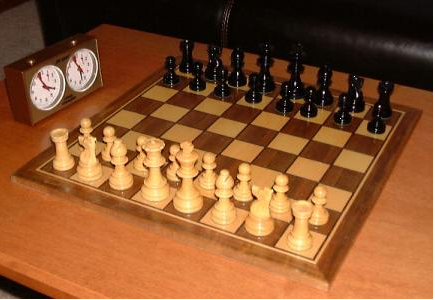
\includegraphics[width=10cm]{images/ajedrez.png}
	\caption{Juego de ajedrez tradicional}
	\label{fig:ajedrez}
\end{figure}

\begin{figure}[h]
	\centering
		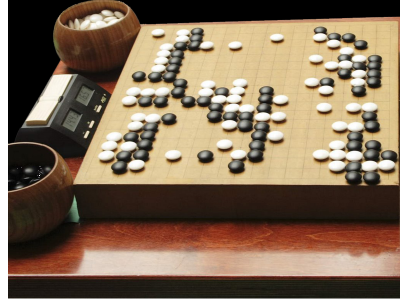
\includegraphics[width=10cm]{images/go.png}
	\caption{Juego de ajedrez chino tradicional o Go}
	\label{fig:go}
\end{figure}

Fij\'andonos en estos dos representantes primigenios de los juegos de estrategia por turnos se puede dar una definici\'on del conjunto: Un juego de estrategia por turnos es aquel en el cual los jugadores disponen de tiempo para meditar su siguiente movimiento (su turno) y que finaliza cuando se realiza dicho movimiento. Es decir en contraposici\'on a los juegos de estrategia en tiempo real, \emph{la acci\'on} se detiene entre cada jugada.
\\
Con estas simples premisas existen infinidad de ejemplos de juegos de tablero que cumplen con esta definici\'on y que son m\'as o menos conocidos: 
\begin{itemize}
	\item \emph{El Risk} se juega sobre un tablero que representa un mapamundi, sobre el los jugadores despliegan fichas que representan sus ej\'ercitos, el objetivo del juego es conquistar una serie de territorios a otros jugadores.
	\item \emph{El Scrabble} es un juego cuyo objetivo consiste en formar palabras sobre un tablero. Para dicho fin, cada jugador recibe un n\'umero espec\'{\i}fico de fichas (o letras), las cuales debe colocar sobre casillas numeradas. Las letras se encuentran igualmente numeradas, y por lo tanto, cada jugador obtiene por cada palabra formada un puntaje que depende tanto del valor de las letras empleadas como de la posici\'on de dichas letras dentro del tablero.
	\item \emph{El Reversi} es un juego entre dos personas, que comparten 64 fichas iguales, de caras distintas, que se van colocando por turnos en un tablero dividido en 64 escaques. Las caras de las fichas se distinguen por su color y cada jugador tiene asignado uno de esos colores, ganando quien tenga m\'as fichas sobre el tablero al finalizar la partida.
\end{itemize}

\subsection{Salto al mundo digital: estrategia por turnos en el PC.}

Los primeros juegos de estrategia por turnos para ordenador fueron, como era de esperar, adaptaciones de los antiguos juegos de tablero. Los retos t\'ecnicos de estos proyectos  se encontraban sobre todo en el apartado de la simulaci\'on y la inteligencia artificial, es decir, en la capacidad de dise\~nar e implementar un sistema que fuera capaz de comportarse como uno o varios jugadores a los que el usuario pudiera enfrentarse. Como an\'ecdota al respecto cabe destacar la \textit{moda} que durante la d\'ecada de los 90 enfrent\'o a superodenadores contra grandes maestros del ajedrez, siendo los m\'as famosos los enfrentamientos entre Gary Kasparov y la computadora de IBM Deep Blue. Actualmente, en cuanto a computaci\'on y ajedrez se refiere se opta por soluciones m\'as enfocadas al software que al hardware (como era Deep Blue) y programas que se pueden encontrar en las estanter\'{\i}as de de las tiendas de videojuegos han sobrepasado el rendimiento de Deep Blue de manera m\'as que notable.\\

\begin{figure}[h]
	\centering
		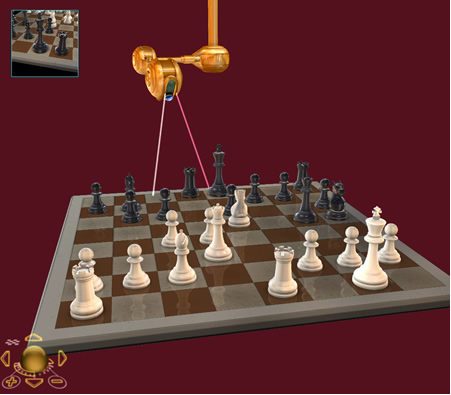
\includegraphics[width=10cm]{images/fritz11.png}
	\caption{Fritz 11, Frans Morsch and Mathias Feist (2007)}
	\label{fig:Imagen de Fritz 11}
\end{figure}
 
Un claro ejemplo de esto es el programa alem\'an Fritz. Por menos de 50 euros cualquiera puede tener en casa un software que ha demostrado su val\'{\i}a derrotando al campe\'on mundial Vladimir Kramnik\footnote{En realidad el programa que venci\'o fue Deep Fritz, una versi\'on optimizada para el uso de procesadores multi-n\'ucleo.}.\\

Pero el medio que brinda el ordenador, m\'as libre de ciertas ataduras f\'{\i}sicas inherentes a los juegos de tablero, pronto comenz\'o a dar como resultado nuevas y m\'as ricas formas de entretenimiento basadas (aun as\'{\i}) en los mismos principios que sus antecesores.\\

Quiz\'as el exponente m\'as claro y con mayor repercusi\'on de la estrategia por turnos dentro del entretenimiento digital sea el \emph{Civilization} de Sid Meier, cuya primera versi\'on data de 1991.\\

\begin{figure}
	\centering
		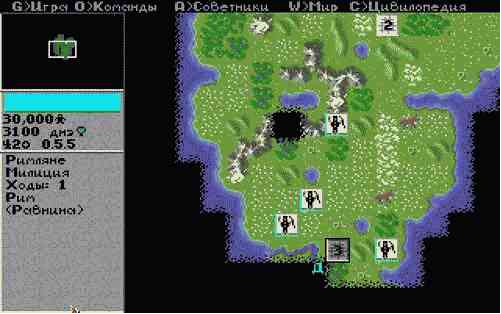
\includegraphics[width=10cm]{images/civilization.png}
	\caption{Civilization, Sid Meier (1991)}
	\label{fig:Imagen de la primera versi\'on para DOS del Civilization}
\end{figure}	
	
En Civilization el jugador toma el rol del regente de una civilizaci\'on empezando con una simple unidad-poblador y trata de construir un imperio compitiendo con otras civilizaciones.\\

El objetivo del juego es dirigir esta civilizaci\'on desde su inicio hasta llegar al espacio o conquistar todo el planeta. Permite ir decidiendo el camino que toman las investigaciones cient\'{\i}ficas,  se puede fundar ciudades, construir y comandar ej\'ercitos, dirigir la construcci\'on de carreteras, elegir la forma de gobierno, mantener relaciones diplom\'aticas con otros pueblos, etc.\\

Existen gran cantidad de versiones de este juego en forma de secuelas oficiales, adaptaciones o incluso una versi\'on completamente libre llamada \emph{FreeCiv}.\\

A partir del Civilization surgieron multitud videojuegos que tomando el concepto trasladaron la acci\'on al espacio exterior (\emph{Master of Orion}, \emph{Ascendancy}), a mundos de fantas\'{\i}a (\emph{Heroes Of Might and Magic}) o a per\'{\i}odos hist\'oricos concretos (\emph{Pirates!}).\\

\subsection{La pol\'{\i}tica en los videojuegos}

Si bien es cierto que el Civilization y sus derivados conten\'{\i}an una gran parte de gesti\'on, su mec\'anica y sobre todo las condiciones del jugador para ganar, exig\'{\i}an que las actividades pol\'{\i}ticas que se pudieran realizar fueran bastante limitadas. En cualquier caso, el objetivo del juego no era el de simular la actividades de un l\'{\i}der pol\'{\i}tico.\\

Para encontrar un juego as\'{\i} tenemos que remontarnos todav\'{\i}a m\'as atr\'as en el tiempo, hasta 1988 con el videojuego \emph{Hidden Agenda}.\\

\begin{figure}[h]
	\centering
		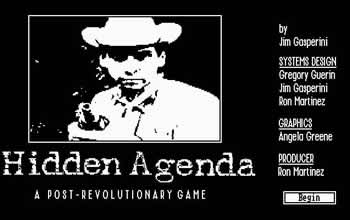
\includegraphics[width=10cm]{images/hiddenAgenda.png}
	\caption{Hidden Agenda, Jim Gasperini (1988)}
	\label{fig:Pantalla inicial de Hidden Agenda}
\end{figure}		
	
En \'el, el jugador asume el papel de un reci\'en electo presidente de un pa\'{\i}s imaginario de Am\'erica latina, reci\'en salido de un r\'egimen dictatorial. La mayor parte del juego se basa en leer textos sobre consejeros pertenecientes a diferentes facciones y tomar decisiones con respecto a estas, tratando de mantener contenta a la mayor parte de la poblaci\'on representada por dichas facciones. Exist\'{\i}a un m\'{\i}nimo componente geopol\'{\i}tico que se manifestaba en la capacidad la alinearse con alguna potencia internacional (EEUU, antigua Uni\'on Sovi\'etica y Europa). Se le considera uno de los precursores del movimiento GamesForChange\footnote{Games for Change (tambi\'en conocido como G4C) es un movimiento y comunidad dedicado al uso de los videojuegos como elemento de cambio social. Se puede encontrar m\'as informaci\'on en us we: http://www.games4change.org }.\\

El ejemplo m\'as contempor\'aneo de juego relacionado con la gesti\'on pol\'{\i}tica es \emph{Democracy}: creado en 2005, el jugador asume el papel de presidente/primer ministro de un gobierno democr\'atico. Las funciones del jugador consisten en introducir y alterar pol\'{\i}ticas en siete areas diferentes (impuestos, econom\'{\i}a, bienestar, relaciones externas, transporte, ley y orden y servicios p\'ublicos). Cada pol\'{\i}tica tienen un efecto en la felicidad de diferentes grupos de poblaci\'on, as\'{\i} como en factores como el crimen o la poluci\'on del aire. 

\begin{figure}[h]
	\centering
		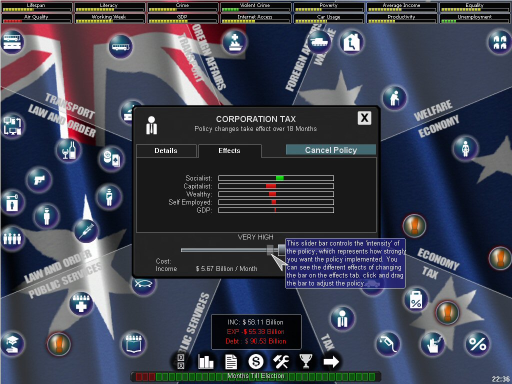
\includegraphics[width=10cm]{images/democracy.png}
	\caption{Democracy, Positech Games (2005)}
	\label{fig:Pantalla de juego de Democracy}
\end{figure}

En principio Democracy puede ser el juego que m\'as  se parezca a HONOS en su planteamiento y concepci\'on. Las diferencias fundamentales radican en que en HONOS se hace mayor hincapi\'e en la intervenci\'on m\'as directa del jugador en ciertos aspectos y no s\'olo a base de pol\'{\i}ticas, as\'{\i} como una mayor complejidad en las relaciones diplom\'aticas.